\subsection{Results} \label{Sec:results}
\headbf{Effectiveness (RQ1)} \figref{assertionTypeFaultDetec} depicts the fault detection rate achieved by (1) \tool, (2) explicit assertions when included individually, and (3) explicit assertions in conjunction with either implicit assertions or (4) candidate assertions. The number on each bar represent the number of faults detected by the corresponding assertion types. As shown in \figref{assertionTypeFaultDetec}, \tool detects on average 62\% of the total faults (ranges from 42-84\%).
The percentage of faults revealed by including only explicit assertions is always less than the ones that are detected through the combination of explicit with either implicit assertions or candidate assertions. This indicates that implicit as well as candidate assertions are essential entities in improving the fault finding capability of \tool. By eliminating implicit and candidate assertions, fault detection rate drops by 27\% on average and up to 31\% for the EnterpriseStore application (ID 2).

\figref{assertionTypeFaultDetec} shows that the improvement brought by implicit assertions is 8\% on average, however, when candidate assertions are included fault detection rate is increased by 21\% on average. This indicates that candidate assertions play a more prominent role in increasing the number of faults detected by \tool in comparison with implicit assertions. Not surprisingly, explicit assertions contribute the most among the other assertion types generated by \tool. Explicit assertions detect 73\% of the total faults on average (ranges from 69-77\%). These assertions are derived directly from the DOM-based oracles written by the developer of the application who has a deep knowledge of the application's behaviour. Therefore, it is expected that code-level assertions derived directly from such oracles have the highest impact on fault finding capability of our tool.        

\begin{figure}[!t]
  \centering
  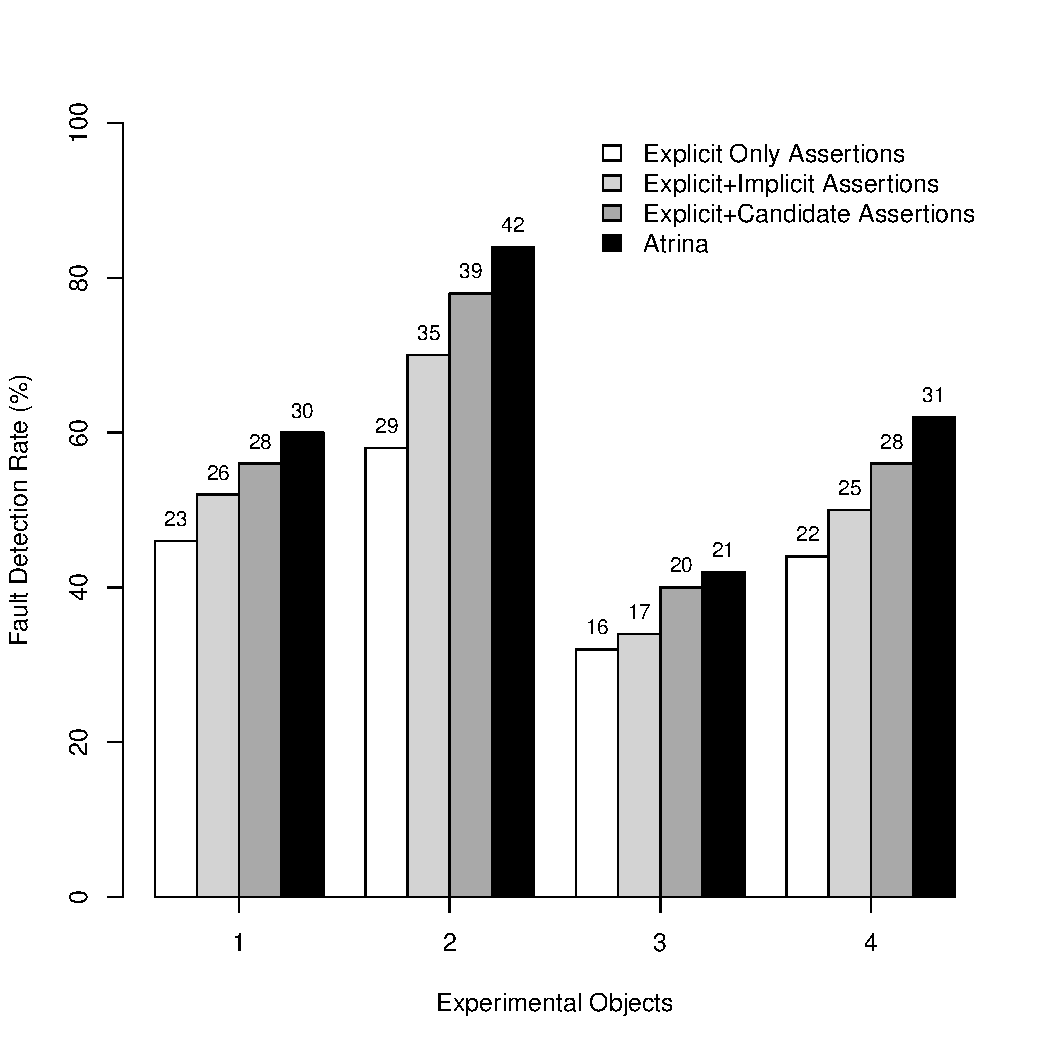
\includegraphics[width=1\hsize]{r-scripts/assertionTypeFaultDetec}
  \vspace{-0.18in} 
  \mycaption{Fault detection rate using different types of generated assertions.}
  \vspace{-0.1in} 
  \label{Fig:assertionTypeFaultDetec}
 
\end{figure}
\headbf{Accuracy (RQ2)}
\tabref{accuracyTable} shows the number of  correctly reported (TP), the number of incorrect reported (FP), and the number of missed (FN) \javascript lines of code, which are related to human-written DOM-based assertions. The table also shows the percentage of precision and recall achieved by \tool. The Recall oscillates between 79 to 100\% (90\% on average). The precision computed for the Phormer (ID 1) and WolfCMS (ID 3) is 100\%. For EnterpriseStore application (ID 2) as well as Claroline (ID 4), the precision rate is 98\%.

We noticed that the lower recall rate obtained by \tool is mainly due to the use of third party libraries. Currently, we focus only on the application source code and do not consider libraries in our slicing technique. The underlying assumption is that faults are mainly originated from the application's code. The small deviation observed in precision is due to the functions, that are called but are not instrumented due to limitations in our current implementation. If the definition of a called function is not instrumented, we assume that the function call is related to our slice, while it may not be. We also observed that in rare cases a variable is seemingly assigned by a return value of a function, though the \code{return} statement is not found in the actual code of the called function. Our current implementation includes such variable assignments in the pertaining slices, which results in a small deviation in the precision.  
\headbf{Comparison with human-written DOM-based Assertions (RQ3)}

\begin{figure}[!t]
  \centering
  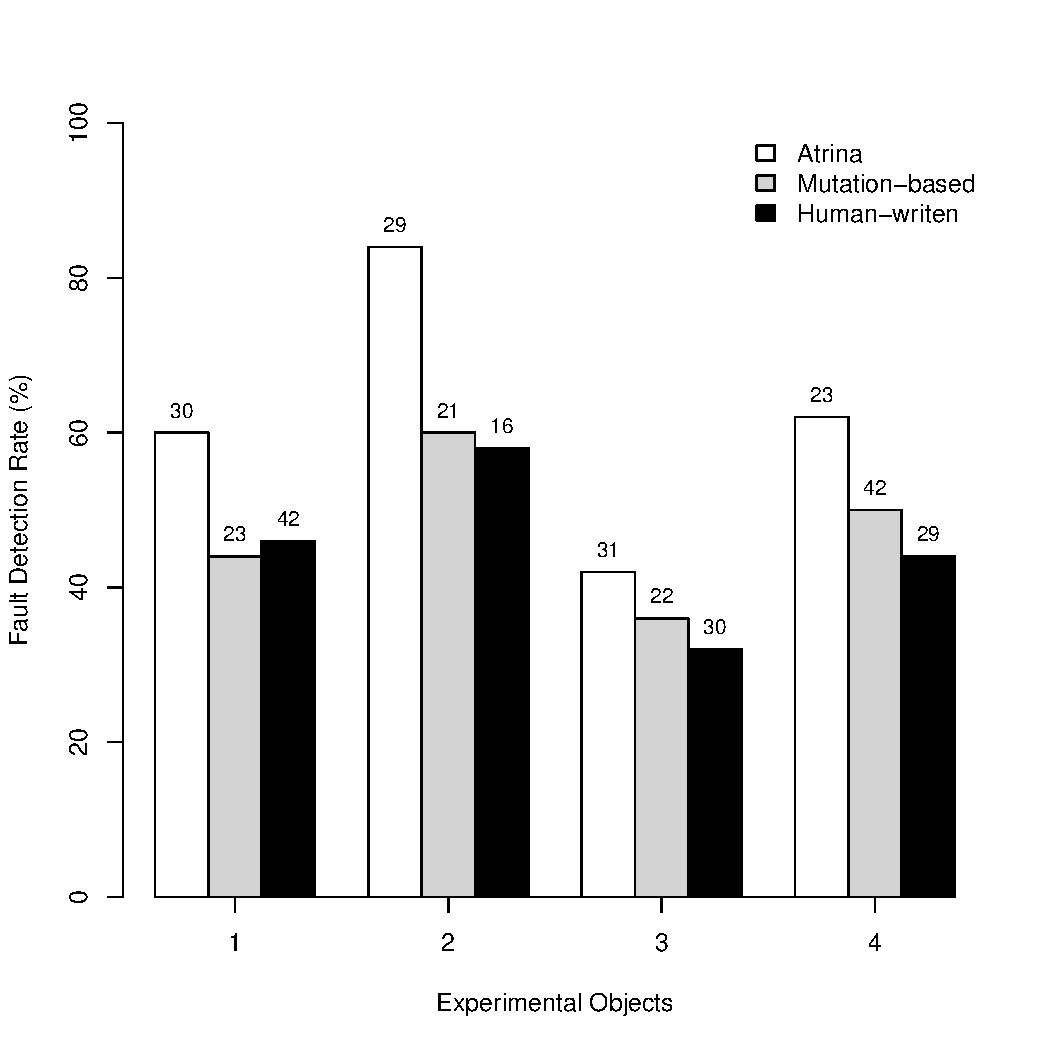
\includegraphics[width=1\hsize]{r-scripts/barplot-faultDetectionRate}
  \vspace{-0.18in}   
  \mycaption{Fault finding capability.}
  \vspace{-0.1in} 
  \label{Fig:faultDetectionRate}

\end{figure}


\begin{table}
        \caption{Accuracy achieved by \tool.} \label{Table:accuracyTable}        
{\scriptsize
\centering
%    \begin{center}
       
      %  \subtable[Experimental subjects and the corresponding exploration data]
            {
           \begin{tabular}{c|c|c|c|c|c||c|c|c|c} \hline
           
&\multicolumn{5}{c||}{\thead{Backward Slice}} & \multicolumn{4}{c}{\thead{Assertions}} \\
\cline{2-10}
          
           
           
\theadturn{App ID} &\theadturn{\# TP (LOC)} &\theadturn{\# FP (LOC)} &\theadturn{\# FN (LOC)} &\theadturn{Precision (\%)} &\theadturn{Recall (\%)} & \theadturn{\# Explicit} & \theadturn{\# Implicit} & \theadturn{\# Candidate} &\theadturn{\# Total}  \\  \hline 
\hline 
1  & 174 & 0 & 0 & 100 & 100 & 41 & 9 & 13 & 63     \\ \hline
           
2 & 861 & 18 & 162 & 98 & 84 & 51 & 19 & 26 & 96    \\ \hline

3 & 193 & 0 & 0 & 100 & 100 & 83 & 23 & 16 & 122   \\ \hline

4 & 1446 & 29 & 385 & 98 & 79 & 72 & 29 & 31 & 132\\ \hline

5 & 1017 & 0 & 224 & 100 & 82 & 78 & 18 & 11 & 107  \\ \hline

6 & 533 & 0 & 0 & 100 & 100 & 24 & 3 & 14 & 41  \\ \hline

7 & 430 & 0 & 0 & 100 & 100 & 14 & 5 & 16 & 35  \\ \hline

AVG & - & - & - & 99.4 & 92.1 & - & - & - & - \\ \hline
\hline\end{tabular}
            }

%\end{center}
}
%\vspace{-0.2in} 
\end{table}
\headbf{Comparison with Mutation-based Assertion Generation (RQ4)}



